\section{Unified Namespace as the Basis for IIoT Systems}
\label{section:unified-namespace}

    % Wie war es früher
    It can be said that the success of a digital transformation strategy depends on how well-integrated organizational data is across business units and technology domains. In \autoref{subsection:automation-pyramid} we discovered that traditional and especially OT-based architectures in the industrial IoT domain have major disadvantages that often make them infeasible in modern systems. We discussed how point-to-point integrations between components of adjacent layers hinder scalability from both the business (high cost for every integration) and the technology (network and performance issues) perspective but also innovation and productivity. These hundreds, if not thousands of point-to-point integrations are a set of implementations only the domain specialists of each integration understand, which almost guarantees to result in technical debt at some point. We also found that this structure leads to data gaps, as only the data necessary for specific integrations is passed around. It also results in data silos, because of data being captured by individual components but not made accessible to other parts of the system. Both of these issues -- data gaps and data silos -- make some use cases like accessing device data from the cloud, which requires integrations between every level, very cumbersome. Lastly, we saw that the heterogeneity of data formats in IIoT is a challenge that needs to be tackled in order to be able to design, develop and maintain a modern IIoT system at scale \cite{hivemq_essentials_uns}.

    % UNS Allgemein
    \begin{figure}[htbp]
        \centering
        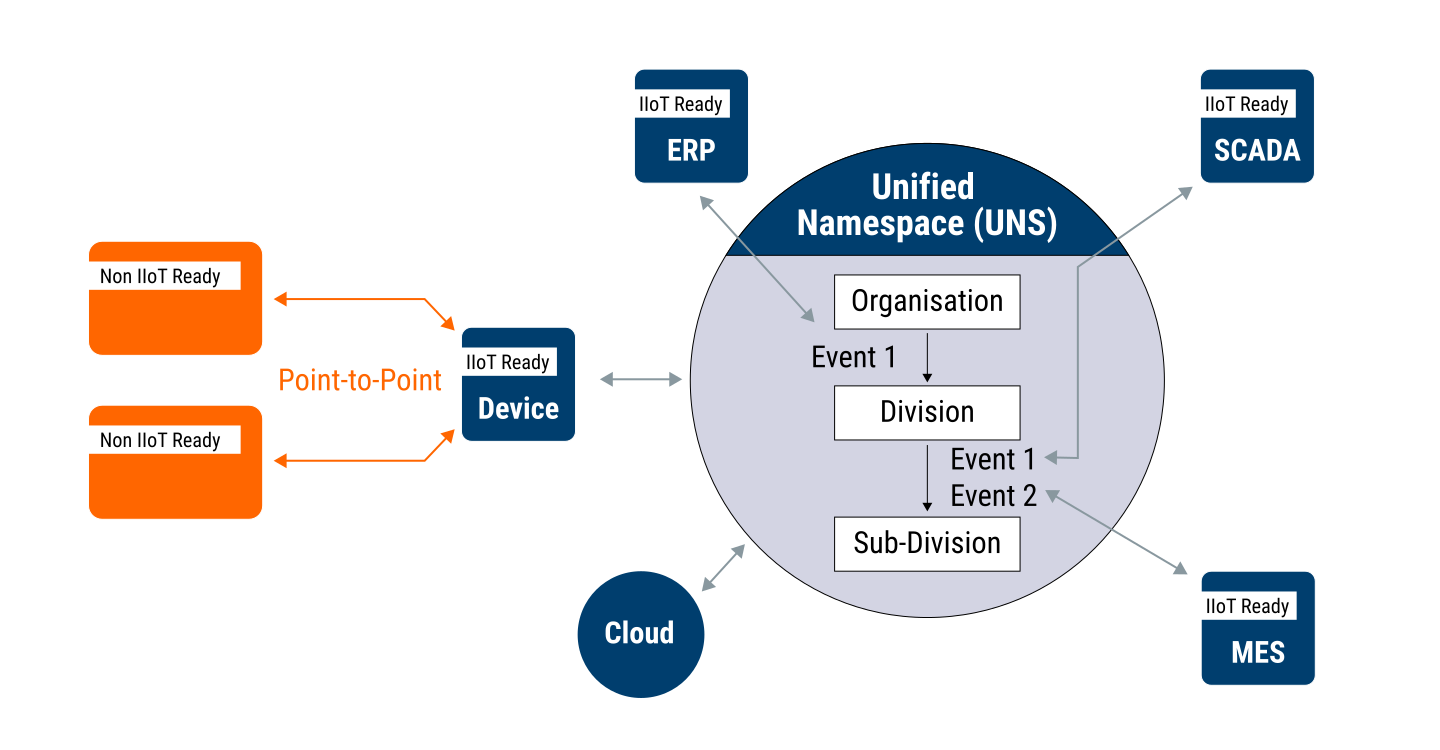
\includegraphics[width=0.9\textwidth]{img/uns-basic-architecture.png}
        \caption{Unified Namespace \cite{hivemq_essentials_uns}}
        \label{figure:hivemq-uns-essentials}
    \end{figure}
    
    \noindent In \autoref{section:common-patterns} we already saw that many more modern architectures follow a pattern where a central message-oriented middleware is used in order to build a uniform basis for data exchange, which has proven to be a more suitable approach for a smart manufacturing or IIoT architecture \cite{smart_manufacturing_using_isa95_mqtt}. Examples of this design are the modern standard ``OPC-UA PubSub over MQTT'' (see \autoref{subsection:opc-ua}) with a central MQTT broker or the ``Microsoft Azure Industrial Internet of Things'' reference architecture which uses the Azure IoT Hub as a central communication node. A modern and increasingly common approach based on this concept is the ``Unified Namespace'' (UNS) which is used in the proposed reference architecture shown in \autoref{figure:mw-reference-arch}. It follows the idea of having all data in a centralized location with a standardized and uniform structure - the unified namespace - and can be seen in \autoref{figure:hivemq-uns-essentials}. This centralized location is a central hub or broker which becomes the single source of truth for the whole IIoT system and is structured in a way that represents the actual structure of the business. A common basis for the structure is the use of ISA-95 layers from the automation pyramid which was discussed in \autoref{subsection:automation-pyramid}. This shows that despite its shortcomings, the automation pyramid can still be complementary to a modern IIoT architecture \cite{smart_manufacturing_using_isa95_mqtt}. After applying the shift of communication structure from point-to-point integrations to a centralized messaging system all components of the system communicate through a central repository of information using a uniform protocol thus solving the issues regarding point-to-point integrations. Components that are not capable of communicating in the uniform protocol are placed behind gateways or adapter/connector services that then bidirectionally communicate with the UNS. The uniform protocol in a system based on the unified namespace must use a publish-and-subscribe (pub-sub) architecture like the standard OPC-UA PubSub with MQTT (\autoref{subsection:opc-ua}) or the protocol MQTT (\autoref{subsubsection:mqtt}), which leads to a loosely coupled, scalable, highly-available and fault tolerant system supporting millions of nodes. Apart from scalability and high availability, the use of this architecture has several beneficial implications. Using this structure, all entities in the system get immediate access to all relevant data by just communicating with the UNS which leads to a simplified integration into the system and thus a reduction of cost since no specialized engineering effort for building custom integrations is required. The ability to access all IIoT data in real-time also enhances development speed, boosts productivity, and opens up greater opportunities for innovation \cite{building_iiot, hivemq_essentials_uns}. \newline

    Let us now look at the requirements that a unified namespace must meet. First of all the UNS should be built upon open-source components in order to assert interchangeability and expandability. The UNS system must also be lightweight since IIoT systems often live in both resource- and network-constrained environments as discovered in \autoref{section:current-situation}. Apart from the edge-driven and push-based approach of the ``PubSub'' architecture which was identified as one of the best communication strategies in IIoT, this can be taken even further by applying ``Report by Exception'' which means that data producers publish data to the UNS only when they detect changes in the monitored value thus reducing network traffic and requirements regarding processing power even further. The following paragraphs will describe how the UNS can be implemented based on the reference architecture shown in \autoref{figure:mw-reference-arch}.\newline

    % Technologien & Sparkplug or not
    The most common open specifications used for implementing UNS projects are MQTT and OPC-UA. In the proposed reference architecture of this thesis, MQTT is used to realize the unified namespace as \autoref{figure:mw-reference-arch} shows. As analyzed in \autoref{subsubsection:mqtt}, MQTT shines through simplicity and understandability which is the main reason why the protocol is chosen in this reference architecture. Its flexible and hierarchical topic structure fits the ISA-95 standard used for structuring the unified namespace perfectly. Following the ISA-95 layers, messages are addressed to the according topics based on the structure ``Enterprise/Site/Area/Line/Cell''. This simplifies the uniform data access even further since data can be accessed or produced by just subscribing or publishing to the desired topic. Even accessing all data of one or more layers of the ISA-95 standard is possible by using MQTT wildcards. Note that while the ISA-95 standard is a common recommendation for the implementation of a unified namespace, a custom structure should be used if the standard does not fit the structure of the business in question \cite{hivemq_essentials_uns}. Regarding performance, MQTT has been proven to fare well when benchmarked against competing protocols like OPC-UA \cite{does_mqtt_uns_solve} and hence represents a solid choice for central communication technology. \newline
    
    In \autoref{subsubsection:sparkplug-b} we discussed the open-source specification ``Sparkplug B'' on top of MQTT which claims to be a framework for seamless integration of applications, sensors, devices and gateways within an existing MQTT infrastructure in a bidirectional and interoperable way. By defining a fixed topic structure, a payload format, a set of commands and a strategy for dealing with state, the specification aims to help with achieving standardization across a large environment, for example an IIoT system. However with the use of Sparkplug B also come disadvantages. First of all the integration of the common standard ISA-95 with hierarchical MQTT topic structures is not compatible with the standardized topic namespaces of Sparkplug B. As a reminder, the Sparkplug B topic namespaces are defined as ``namespace/group\_id/message\_type/edge\_node\_id/device\_id''. To tackle this issue, Sparkplug B provides two distinct methods. The ``Parris Method'' by Matthew Parris fits the entire ISA-95 structure into the ``group\_id'' level of the Sparkplug B topic namespace by using a custom delimiter rather than the topic delimiter ``/'' of MQTT which might for example look like ``spBv1.0/Plant1:Area3:Line4:Cell2/NDATA/edge1.2.1'' where the ``namespace'' field is set as the ``Enterprise'' level of ISA-95. While this provides a simple fix for combining ISA-95 and Sparkplug B, it falls short since MQTT does not support publishing or subscribing to substrings. This means that applications can for example no longer subscribe to all data of a production site with a wildcard directly, but need to subscribe to all topics of the namespace (in this case ``spBv1.0/\#'') and destructure messages themselves thus resulting in much higher data volume and use of computational power. The other method provided by Sparkplug B is the ``Schultz Method'' developed by David Schultz which doesn't just use a single broker but multiple brokers at various levels (e.g. Area, Line, Cell) of the enterprise to build the UNS. Lower-level brokers will publish their data to the higher-level broker to achieve a single source of truth in the end again. While this method is also feasible, it again adds lots of additional complexity and operational overhead. 
    
    Another issue is that Sparkplug B uses Protobuf as the encoding for the payload. Although it offers greater technical efficiency, the binary encoding used by Protobuf lacks the human readability of the industry-standard JSON. In the realm of IIoT, where data frequency is often a more significant concern than data volume, the larger size of a JSON message is usually not an issue. More drawbacks include the fixed Quality-of-Service levels defined in Sparkplug B which might not fit every use case, the limited command set which misses common use cases like backfilling historical data and the lack of a specification about time series compression \cite{building_iiot, hivemq_essentials_uns, does_mqtt_uns_solve}. Since Sparkplug B shows several shortcomings when it comes to implementing a unified namespace for an IIoT system, and its useful features can be implemented when needed anyway, plain MQTT is chosen in favor of Sparkplug B in this reference architecture.

    \begin{figure}[htbp]
        \centering
        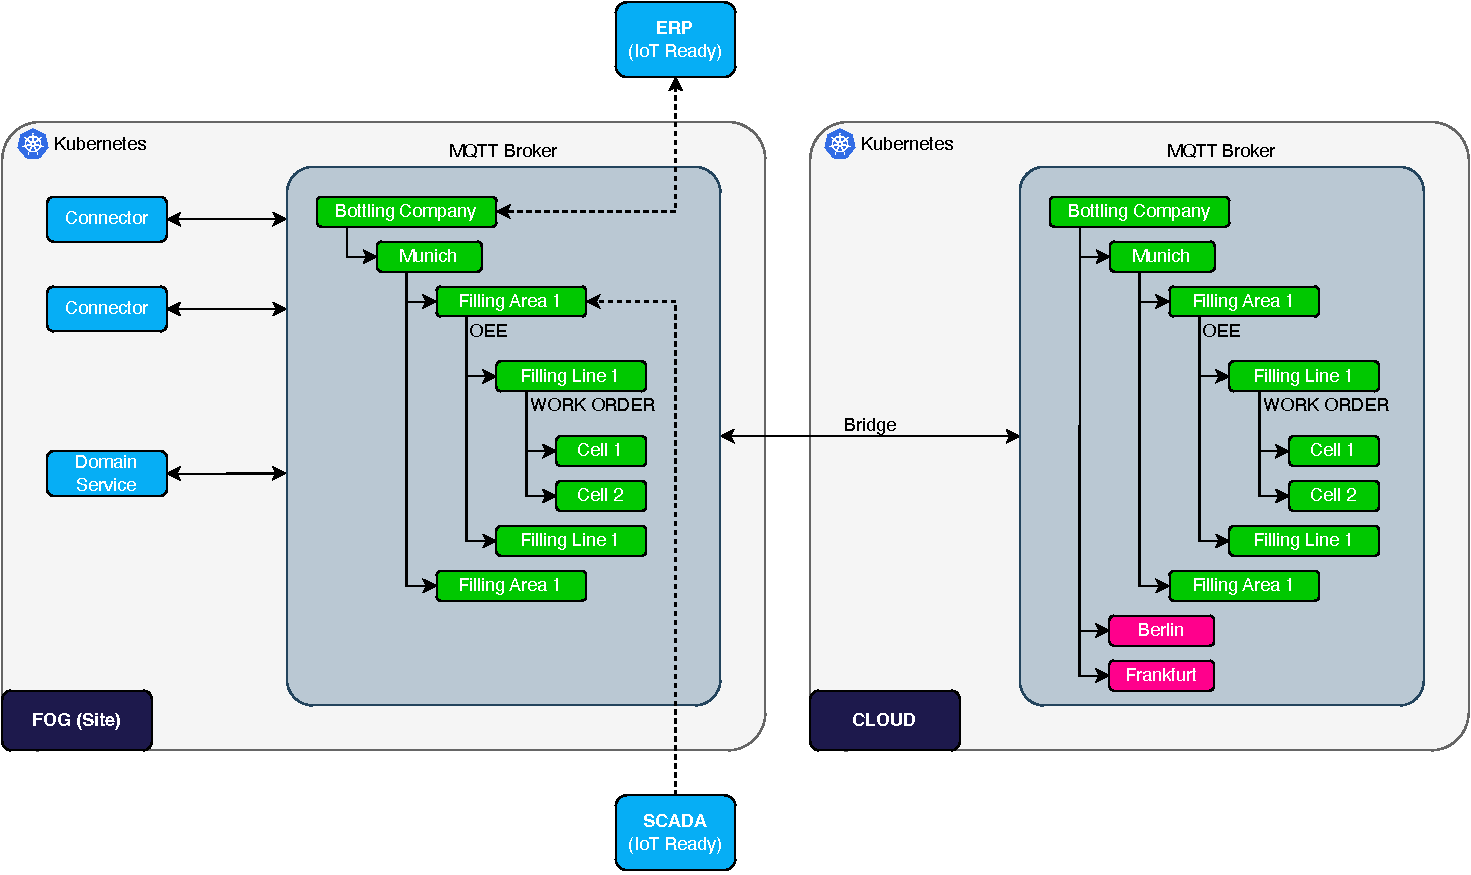
\includegraphics[width=\textwidth]{img/UNS_Reference_Implementation_Strategy_bold.pdf}
        \caption{Concrete UNS implementation following the reference architecture \cite{building_iiot}}
        \label{figure:uns-impl-strategy}
    \end{figure}

    \noindent Next, we explore how the implementation of the UNS is realized when following the proposed reference architecture. \autoref{figure:uns-impl-strategy} shows one fog environment (left) and the central cloud environment (right) of an exemplary implementation. Starting with the fog environment, we can see the sample structure of the UNS realized within an MQTT broker based on the hierarchical ISA-95 topic structure. The graphic not only illustrates how devices interact with the UNS through connectors, but also shows how common IIoT components (see \autoref{subsection:automation-pyramid}) can easily connect to the IIoT system by consuming and/or producing data to topics of interest in the UNS. Examples of this are a SCADA system, that subscribes to all data required to run the production and publishes commands back to the UNS for others to receive, or an ERP system, that subscribes to the data of the whole production site in order to calculate and publish key performance indicators (KPI) \cite{hivemq_essentials_uns}. Since this environment runs fully on-premises, every IIoT component or service can instantly access the production site's data, avoiding the latency associated with communication to the cloud environment. The figure also shows that the cloud system also hosts a unified namespace based on an MQTT broker. This strategy is called ``layered databus'' and was already mentioned in the IIRA in \autoref{subsubsection:iira}. The idea here is, that each production site has its own UNS for the communication within the site. Even if the connection to the cloud were to be disrupted, the production site would remain operational. The MQTT brokers representing the unified namespaces of the production sites forward their data to the central MQTT broker using an MQTT bridge, which consumes all topics of the production site broker and publishes the messages to the same topics on the cloud broker. Note that depending on the use case, it might be desirable to use a technology with even stronger message delivery guarantees like Apache Kafka for the bridge between the on-premises sites and the cloud. This reference architecture chooses MQTT over Kafka mainly for standardization purposes across a large ecosystem. The cloud broker, serving as the enterprise-wide single source of truth, enables workloads operating in the cloud environment to efficiently perform operations on extensive enterprise data by simply subscribing to the topics of interest. Additional supporting tools, such as data streaming applications like Apache Kafka, and long-term storage databases like TimescaleDB or OpenSearch, can also process or persist the data managed by the central cloud broker. Note that the data in the cloud broker may not be the most recent due to latencies or even connectivity issues, which is why low-latency workloads should run in the fog or even the edge environment. The MQTT bridge can be implemented bidirectionally, enabling use cases such as issuing commands from the cloud to edge devices. Executing a command becomes as straightforward as publishing a message to the appropriate topic in the cloud environment. This message is then seamlessly forwarded through the bridge to the on-premises MQTT broker, where the corresponding edge device can receive it \cite{building_iiot}.
    